\documentclass[12pt,a4paper]{report}

\usepackage[a4paper,margin=2.5cm]{geometry}
\usepackage{graphicx}
\usepackage{xcolor}
\usepackage{array}
\usepackage[hyphens]{url}
\usepackage{setspace}
\usepackage{enumitem}
\usepackage{tikz}
\usepackage{caption}

\setstretch{1.15}
\setlength{\parindent}{0pt}
\setlength{\parskip}{0.6em}
\urlstyle{same}
\Urlmuskip=0mu plus 2mu
\captionsetup{font=small,labelfont=bf}

\newcommand{\groupname}{Group 20}
\newcommand{\supervisor}{Dr.\ Dragule Swaib}
\newcommand{\supervisoremail}{dragule@gmail.com}

\newcommand{\doctype}{Project Proposal}
\newcommand{\doctypelower}{project proposal}
\begin{document}
%-------------------------------------------------- Cover page
\begin{titlepage}
\centering
\vspace*{0cm}

\includegraphics[width=0.97\textwidth]{logo-000.png}\par
\vspace{1.2cm}
{\LARGE\bfseries A smart bin system for classification, fill-up\\prediction and smart disposal\par}
\vspace{0.8cm}
by\par
\vspace{0.5cm}
{\large\groupname}\par
\vspace{0.7cm}
{\large\bfseries Department of Computer Science\\
School of Computing \& Informatics Technology\par}
\vspace{0.7cm}
{\itshape A \doctype{} Submitted to the\\
School of Computing and Informatics Technology for the Study Leading to a\\
Project Report in Partial Fulfilment of the requirements\\
for the Award of the Degree of Bachelor of Science in\\
Computer Science of Makerere University\par}
\vspace{0.8cm}
{\large\textbf{Supervisor:}\\
\supervisor\par}
\vspace{0.4cm}
Department of Computer Science\\
School of Computing \& Informatics Technology\\
\supervisoremail\par
\vspace{0.6cm}
October, 2026\par
\end{titlepage}

%-------------------------------------------------- Front matter
\pagenumbering{roman}

\chapter*{Declaration}
\addcontentsline{toc}{chapter}{Declaration}

We, Group \groupname, declare that this \doctypelower{} is our own original work. It has not been published, and it has not been submitted to any other university for the award of a degree.

\vspace{0.8em}
\renewcommand{\arraystretch}{2.1}
\begin{tabular}{@{}c>{\raggedright\arraybackslash}p{5.3cm}l>{\raggedright\arraybackslash}p{3.4cm}@{}}
\hline
\textbf{No.} & \textbf{Names} & \textbf{Registration Number} & \textbf{Signature}\\
\hline
1 & Nambirige Eron & 24/U/1026 & \\
2 & Nagawa Sandra Robinah & 24/U/08037/PS & \\
3 & Nakimuli Jollyne Flavia & 24/U/0953 & \\
4 & Malual Martin Biar & 24/E/21484/PS & \\
\hline
\end{tabular}
\renewcommand{\arraystretch}{1}

\vspace{1.5em}
Date: \dotfill\hspace{4cm}

\chapter*{Approval}
\addcontentsline{toc}{chapter}{Approval}

This \doctypelower{} is submitted for examination with the approval of the following supervisor.

\vspace{2em}
Signed: \dotfill\hspace{4cm}

\vspace{1.2em}
Date: \dotfill\hspace{4cm}

\vspace{2em}
\supervisor\\
School of Computing \& IT\\
College of Computing \& IT\\
Makerere University\\
\supervisoremail

\chapter*{Dedication}
\addcontentsline{toc}{chapter}{Dedication}

We dedicate this \doctypelower{} to our parents and guardians, who have supported us throughout our studies.

\chapter*{Acknowledgement}
\addcontentsline{toc}{chapter}{Acknowledgement}

We thank our supervisor, \supervisor, for guiding us as we developed this project. We are also grateful to the members of our group, whose discussions shaped the system we are proposing.

\tableofcontents

\clearpage
\listoffigures
\addcontentsline{toc}{chapter}{List of Figures}
\listoftables
\addcontentsline{toc}{chapter}{List of Tables}
\chapter*{List of Abbreviations}
\addcontentsline{toc}{chapter}{List of Abbreviations}
\begin{tabular}{@{}p{2.6cm}p{10cm}@{}}
CNN & Convolutional neural network\\
GSM & Global System for Mobile Communications\\
IoT & Internet of Things\\
KCCA & Kampala Capital City Authority\\
LSTM & Long short-term memory\\
LTE & Long-Term Evolution\\
MAE & Mean absolute error\\
MAPE & Mean absolute percentage error\\
RMSE & Root mean square error\\
\end{tabular}
\clearpage
\pagenumbering{arabic}
\chapter{Introduction}

This chapter explains why we are proposing a smart bin system. It starts with how waste management in Kampala has reached its present state, moves to the problem that follows from this, and then gives the objectives, the scope and the significance of the study.

\section{Background}

Managing waste involves more than taking rubbish out of a bin. The waste has to be separated, stored, collected and taken to a suitable place, and when these steps are poorly connected, materials that could have been recovered end up mixed with everything else. The World Bank estimated that the world produced 2.01 billion tonnes of municipal solid waste in 2016 and expects 3.40 billion tonnes by 2050 \cite{kaza}.

Kampala shows the problem at city level. KCCA puts the waste generated in the city at over 2,500 tonnes a day \cite{kcca2026}. Mwesigwa \cite{mwesigwa} reports that about 1,200 tonnes a day are collected by garbage trucks, which is roughly 48 percent, and that KCCA's own collection rate rose from 35 percent in 2016 to 59 percent in 2023. KCCA reported 65 percent for the 2023/2024 financial year \cite{kcca2024a}. These figures are not the same because they are measured in different ways, but they all show that a large part of the waste is never collected. Waste that is left behind often ends up in drainage channels and on roads, where it blocks water and causes flooding \cite{ngwomoya,mwesigwa}.

The reasons for the gap have built up over several years. Collection is shared between KCCA and private contractors \cite{kccand}. Reports on the arrangement mention too few trucks and frequent breakdowns, limited funding, contractors who collect on irregular schedules or overcharge, and residents who do not pay collection fees \cite{ngwomoya,mwesigwa}. The city has also kept growing. KCCA lists population growth, economic growth and rising waste generation among the reasons its main landfill filled up \cite{kcca2026}.

Most of the waste is also not separated at source. KCCA's own figures put the composition at about 85 percent organic waste, 8 percent plastic, 2 percent paper and 5 percent other material \cite{kcca2026}. Material with a use, such as food waste that could go to farms or compost, is therefore likely to be carried to the same dump as everything else. KCCA has asked people to separate organic and inorganic waste at source \cite{kccand}. Okello \cite{okello} names low public awareness, weak enforcement and a lack of reliable data among the problems, and Mwesigwa \cite{mwesigwa} suggests that degradable waste could be used to produce biogas.

The Kiteezi landfill is where these problems ended up. It opened in 1996 on 39 acres and was receiving about 1,200 tonnes a day when it was closed \cite{kcca2026}. According to Mwesigwa \cite{mwesigwa}, it had run for about ten years longer than it was meant to, and Africanews \cite{africanews} reports that plans to move waste disposal elsewhere had stalled since 2016. After heavy rain in August 2024 a large part of the waste mound collapsed onto the houses next to it \cite{petley,okello}. KCCA reported that at least 35 people died \cite{kcca2024b}. A year later the site was no longer in official use but was still giving off methane, and disposal had moved to a new site in Mpigi that the National Forestry Authority said encroaches on a protected area \cite{afp}. Among the reforms Okello \cite{okello} recommends are waste diversion strategies and more awareness of waste separation. We take from this that a lot of what reaches the dump could have been kept out of it if it had been separated and collected on time at the places where it is produced.

The Internet of Things (IoT) connects physical devices that take measurements to other systems that can use them. For waste, Medvedev et al. \cite{medvedev} describe a decision support system that combines RFID tags, sensors, cameras and actuators so that truck drivers can share information in real time and routes can be changed as conditions change. In smart bins, fill-level sensors report how much space is left. Ahmed et al. \cite{ahmed} used time series from IoT-connected municipal bins to forecast the status of bins with four deep learning models, and found that an LSTM model gave the lowest percentage error (MAPE of 1.855). Image classification has also been moved onto small devices. White et al. \cite{white} report an accuracy of 0.970 on the TrashNet test set with a model designed to run on a Jetson Nano. Li and Grammenos \cite{li} report 95.98 percent on a seven-class test set with a MobileNet V3 model on the same board, running at 40 inferences a second, and show a cheaper K210 board that uses far less power. These results come from their own datasets and conditions, so we cannot assume the same figures for hotels and restaurants in Uganda.

Some smart bin work has already been done locally and in the region. Musoke \cite{musoke} describes a prototype with fill-level sensors, material detection and reporting to a cloud platform, and Turyahebwa \cite{turyahebwa} describes camera-based identification, sorting into compartments and remote reporting over LTE. Both are Makerere projects, and we have only seen the repository abstracts. They show that this kind of work exists locally, but not how well the prototypes performed or whether they were ever used outside the lab. We will read the full reports during the study of the current situation. Kwagala and Badoru \cite{kwagala} propose a smart municipal waste system for Kampala that uses smart bins for billing and route optimisation, but the results in their abstract are expected results and were not yet measured. Komane and Mathonsi \cite{komane} design a system for Johannesburg with ultrasonic sensors, GPS and GSM, and report no measured accuracy for it.

The image data also has to match the waste classes we plan to use. TrashNet has 2,527 images of glass, paper, cardboard, plastic, metal and general trash, but nothing labelled as organic \cite{yang,white}. It may help with early experiments on some classes, but we will have to collect our own images, especially of food waste and of items photographed under the conditions the prototype will work in.

We chose hotels and restaurants because they prepare food and use a lot of packaging. The preliminary study will establish which types of waste the participating sites produce, how their staff separate it and how collection is arranged. We will also look at space, cleaning, electricity and network access, since a bin that is hard to use or keep clean may be ignored even if its electronics work.

Our proposed system brings classification, compartment monitoring, fill-up prediction and collection support together in one prototype. A mobile application will show the status of the bin, alert authorised collectors and record where the separated waste is taken. By smart disposal we mean sending each recognised item to the right compartment and arranging for it to be taken to a suitable recipient. We are not claiming that the bin treats the waste itself, or that every item can be recycled.

\section{Problem statement}

The background points to a chain of problems. Waste in Kampala is mostly not separated at source, a large share of it is not collected at all, and what is collected goes to a small number of disposal sites. Hotels and restaurants produce food waste and packaging every day, and unless the waste is separated where it is produced, material that could be recovered is mixed again and joins the rest. The collectors who serve these sites work on schedules that have been reported as irregular \cite{mwesigwa}, and they have no way of knowing how full a bin is before they arrive. We expect that bins at some sites are overflowing when the collector comes, while others are emptied when they are half full, and we will check this at the selected sites through observation and interviews. We do not assume that the situation is the same across Uganda.

Earlier prototypes show that automatic identification and remote monitoring can be done. The sources we have seen, however, do not show a prototype that combines four-class sorting, a separate fill level for each compartment, a prediction of the time until a collection threshold is reached, and a record of where the separated waste goes, tested in hotels and restaurants in Uganda. Several of them report no measured results or only results from open datasets. The specific problem of this study is therefore the lack of timely, per-compartment information on what waste has been separated, how full each compartment is and when it will need to be collected. We will develop and test a workflow that supplies this information to hotel staff and collectors under the conditions at selected sites.

\section{Main objective}

To develop and evaluate a smart bin system for waste classification, fill-up prediction and smart disposal in selected hotels and restaurants in Uganda.

\subsection{Specific objectives}

\begin{enumerate}[leftmargin=*,itemsep=0.4em]
\item To study current waste handling practices, collection arrangements and existing smart bin systems at selected hotels and restaurants in Kampala.
\item To analyse the requirements of the proposed system and specify its functional and non-functional requirements.
\item To design the bin, the sorting mechanism, the data storage, the prediction component and the mobile application based on the requirements.
\item To implement a prototype that classifies organic, plastic, paper and glass waste, monitors compartment fill levels, predicts the time to a collection threshold, and supports collection alerts and disposal records.
\item To test and evaluate the prototype in terms of classification performance, sorting success, fill-level measurement error, prediction error, alert delivery time and how well users complete collection tasks.
\end{enumerate}

\section{Scope of the study}

\subsection{Geographical and user scope}

The study will focus on selected hotels and restaurants in Kampala, Uganda, subject to permission and access. The participants will be staff who handle waste, collection personnel, and people who could receive the separated materials. The prototype will first be tested in a controlled setting, before any supervised trial at a site. Airports remain a possible future application, but we have left them out of the first prototype to keep the study manageable.

\subsection{System scope}

The prototype will take one supported item at a time and try to classify it as organic, plastic, paper or glass. A camera and a small computing unit will handle classification, and a controller will run the sorting mechanism and the compartment sensors. The final hardware will be chosen during design. We will not assume that any single unspecified sensor can reliably tell organic waste or plastic apart. Items that are not recognised, are mixed, or are classified with low confidence will be held for manual checking, and the bin will not sort anything into a compartment that is already full.

Fill level will be measured separately for each compartment. Time-stamped readings and emptying events will be stored to support prediction. The prediction will be an estimate of the time remaining before a configurable collection threshold is reached, not a claim about exactly when the bin will overflow. A simple estimate based on the recent fill rate will be the baseline against which the prediction model is evaluated. Where there is not enough history, the application will show the current fill level and threshold alerts, and will not present a forecast it cannot support.

The mobile application will show fill levels, predictions and alerts. Authorised users will be able to acknowledge collection requests and record the collection time, the waste category and the recipient. Suitable organic material may be offered to composting or other approved recovery users once we have confirmed what they will accept. Plastic, paper and glass will only be offered to recipients who accept those materials. The application will record these transfers, but it will not guarantee a market or arrange the physical transport.

\subsection{Study boundaries}

The study covers the study of the current situation, requirements analysis, design, implementation and evaluation within the academic project period. It leaves out hazardous and medical waste, liquids, metal sorting, large mixed loads, vehicle route optimisation and payment services, and it will not attempt citywide deployment. Classification and prediction will be assessed on data kept apart from the training data. For prediction, we will test on later observations so that the model is not judged on its own training history. If the data collection period turns out to be short, we will state this as a limitation of the findings.

\section{Significance of the study}

For waste handlers, meaning the staff of hotels and restaurants and the collection personnel, the prototype may make it easier to separate the supported types of waste and to see which compartments need attention. Current fill levels and estimated collection times may help collectors decide which sites to visit first, and the acknowledgement and collection records will let staff tell the difference between an alert that has been received and a bin that has actually been emptied. Any improvement in collection timing will have to be shown during testing.

For local authorities such as KCCA, records of waste categories, quantities and collection times from participating sites could fill part of the data gap that Okello \cite{okello} points out. KCCA has already asked for separation at source \cite{kccand}, and a site that separates its waste and records where it goes gives the authority something it can check. The study will also show whether this kind of monitoring is practical before anyone proposes it for more sites.

For the users of the system, which are the hotels and restaurants themselves, the study will show whether automatic sorting is practical in a place where items may be dirty, damaged or hard to recognise. It will also give them a record of what they throw away and who collects it, which they can use in their own planning.

For the environment, the benefit depends on how much of the waste is really separated and recovered. If food waste goes to farms or composting and recyclable material goes to recipients who accept it, less of it ends up in a landfill. The collapse at Kiteezi shows what happens when a disposal site is overloaded, so reducing what is sent there matters. The benefit will depend on what each recipient is willing to accept, and the study will look into those conditions before proposing any transfers.

For researchers and students, the project will produce a documented prototype and evaluation results that show both what it can do and where it falls short. Classification precision and recall, the proportion of items routed correctly, fill-level error, prediction error and alert delivery time will give measurable evidence. The findings may help guide later work on waste management systems that suit local operating conditions.

\chapter{Literature Review}

\section{Introduction}

This chapter reviews the studies that bear on the proposed smart bin system. It looks at how waste management problems have been approached with IoT, how waste can be classified by image, how bin fill level can be measured and predicted, and what existing smart bin systems have shown. The chapter ends by stating the gap our project addresses and the parameters we will use to judge the prototype.

\section{Waste management and the role of IoT}

Chapter 1 described a collection system in Kampala that leaves a large share of the waste uncollected, mixes most of what it collects and sends it to a landfill that failed in 2024. The literature on smart cities treats efficient waste collection as a basic service and looks at IoT as a way to improve it. Medvedev et al. \cite{medvedev} propose a decision support system built from RFID tags, sensors, cameras and actuators. In their design, truck drivers share information in real time and collection routes are changed dynamically. They also use cameras to record places that are not being served so that the authorities have evidence. Their work is about the collection side of the problem. It does not deal with separating the waste where it is produced, which is where our project starts.

Okello \cite{okello} writes about Kampala after the Kiteezi collapse and lists the lack of data on collection among the weaknesses of the system, together with divided responsibility, weak enforcement and low public awareness. This is a useful link to IoT. A device that records what is thrown away and when a bin is emptied produces the kind of data she says is missing, although one bin is only a small part of the city.

\section{Waste classification}

Waste classification is usually treated as an image classification problem. The dataset most often used is TrashNet, which has 2,527 images in six classes (glass, paper, cardboard, plastic, metal and trash) \cite{yang,white}. It has no organic class. This matters for Kampala, where KCCA puts about 85 percent of the waste in the organic category \cite{kcca2026}. A model trained only on TrashNet could not identify most of the waste in the city, so a project in this setting has to collect its own images of food waste.

White et al. \cite{white} built WasteNet by applying transfer learning to a DenseNet model pre-trained on ImageNet. They trained only the top layer first and then unfroze the rest gradually. On the TrashNet test set the model had an accuracy, precision, recall and F1 of 0.970, ahead of DenseNet169 at 0.953 and AlexNet at 0.784. The model was designed to run on a Jetson Nano without a cloud connection. The paper does not report inference time or power use, so it says little about how practical the model is on a bin. The result also comes from a split of a single public dataset, so it does not tell us how the model would do on waste photographed in a different place.

Li and Grammenos \cite{li} went further on the hardware side. They trained MobileNet models on TrashNet plus about 1,800 images they collected themselves, which included two extra classes, hand and empty. On a Jetson Nano their MobileNet V3 model reached 95.98 percent on a seven-class test set and ran at 40 inferences a second in the 5 W power mode. On a K210 board the MobileNet V1 model reached 95.58 percent on the same seven classes, used 0.89 W and took 66 ms per inference. They give the cost of the K210 board as about GBP 23 against GBP 133 for the Jetson Nano. The extra classes are worth noting for our design, because they let the bin avoid classifying an empty chamber or a hand reaching in. The paper also claims that the bin could raise the recycling rate in the UK to 95 percent, but nothing in the paper tests this, so we do not rely on it.

Taken together, these papers show that small models can classify waste accurately on low-power hardware. They also show the limits of the evidence. The accuracy figures come from datasets that are cleaner and have fewer classes of mixed food waste than a hotel kitchen would produce, so we treat them as an upper reference rather than as a target we are sure to reach.

\section{Fill-level monitoring and prediction}

The usual way of measuring fill level is with an ultrasonic sensor mounted in the lid. Komane and Mathonsi \cite{komane} use HC-SR04 sensors, which have a range of 2 cm to 400 cm, in pairs so that one can back up the other, together with GPS and a GSM link. They claim that the readings are 99 percent correct when both sensors agree, but they give no test data, so this is a design argument and not a measured result. For our bin, each compartment will need its own sensor, and the measurement error will have to be checked against a ruler because waste surfaces are uneven.

Prediction is a separate step from measurement. Ahmed et al. \cite{ahmed} forecast the status of municipal bins from IoT time series using a 1D CNN, an LSTM, a GRU and a Bi-LSTM. They compared the models using MAE, MAPE, R\textsuperscript{2} and RMSE. The 1D CNN had the lowest RMSE (1.12) and the LSTM the lowest MAPE (1.855), and the authors recommend the LSTM. Their bins were public municipal bins, and the data came from sensors in the field, which is closer to our situation than an image dataset is. A hotel kitchen will have a different pattern, with peaks around meals and deliveries, and we expect to have far less history than a long-running municipal deployment. For this reason we will compare any learned model with a simple baseline based on the recent fill rate, and fall back on threshold alerts when there is not enough data.

\section{Existing smart bin systems}

Table~\ref{tab:existing} summarises the systems discussed in this review and in Chapter 1. The last column states what the source does not show.

\begin{table}[htbp]
\centering
\small
\renewcommand{\arraystretch}{1.25}
\begin{tabular}{>{\raggedright\arraybackslash}p{2.6cm}>{\raggedright\arraybackslash}p{4.9cm}>{\raggedright\arraybackslash}p{5.6cm}}
\hline
\textbf{Source} & \textbf{What it does} & \textbf{What it does not show}\\
\hline
White et al. \cite{white} & Edge classification of six TrashNet classes with transfer learning; 0.970 accuracy & No organic class, no inference time or power, no fill monitoring\\
Li and Grammenos \cite{li} & Edge classification on Jetson Nano and K210; 95.98\% and 95.58\% on seven classes; power and cost compared & No fill-level monitoring or collection support; the recycling-rate claim is not tested\\
Ahmed et al. \cite{ahmed} & Forecasts bin status from IoT time series with four deep learning models & Does not classify waste; public bins, not hotels or restaurants\\
Komane and Mathonsi \cite{komane} & Design with ultrasonic sensors, GPS, GSM, cameras and a user app, for Johannesburg & No measured accuracy or test results\\
Kwagala and Badoru \cite{kwagala} & Smart bins and analytics for routes and billing in Kampala & Results given are expected, not measured (abstract only)\\
Musoke \cite{musoke} & Fill-level sensors, material detection and cloud reporting (Makerere) & Performance and deployment unknown (abstract only)\\
Turyahebwa \cite{turyahebwa} & Camera identification, sorting into compartments, LTE reporting (Makerere) & Performance and deployment unknown (abstract only)\\
\hline
\end{tabular}
\caption{Existing smart bin work reviewed}
\label{tab:existing}
\end{table}

\section{Gap and justification of the proposed solution}

From the sources we reviewed, the pieces of the proposed system exist separately. Classification at the edge has been shown on open datasets, fill-level measurement and forecasting have been shown on municipal bins, and two Makerere projects and one Busitema dissertation work on smart bins in Uganda. What we did not find is a single prototype that (a) classifies organic, plastic, paper and glass waste with its own food-waste images, (b) measures the fill level of each compartment, (c) predicts the time to a collection threshold and compares it with a simple baseline, and (d) records the handover to a recipient, with all four tested in hotels or restaurants in Uganda and reported with measured results. We have not read the full Makerere reports, so this gap may be narrower than the abstracts suggest. We will check this during the study of the current situation.

The case for the proposed solution rests on three points from the literature. First, the problem is real and documented locally: low collection rates, mixed waste, and a landfill collapse that cost lives \cite{mwesigwa,kcca2024b,petley}. Second, the technology is mature enough to build a prototype at low cost, as Li and Grammenos \cite{li} show for the hardware. Third, the evidence does not carry over to our setting, because the datasets lack organic waste and the reported accuracies are from conditions that are easier than a kitchen. A prototype tested on site is the way to find out.

\section{Evaluation parameters}

The literature uses accuracy, precision, recall and F1 for classification \cite{white,li} and MAE, MAPE, R\textsuperscript{2} and RMSE for forecasting \cite{ahmed}. We add parameters for the physical and user side of the system. Table~\ref{tab:params} lists the measures we will use. The targets are our own proposals, chosen with the reported results in mind but set lower where our conditions are harder, and we will confirm them with our supervisor before testing starts.

\begin{table}[htbp]
\centering
\small
\renewcommand{\arraystretch}{1.25}
\begin{tabular}{>{\raggedright\arraybackslash}p{3.0cm}>{\raggedright\arraybackslash}p{5.4cm}>{\raggedright\arraybackslash}p{3.5cm}}
\hline
\textbf{Parameter} & \textbf{How it will be measured} & \textbf{Proposed target}\\
\hline
Classification accuracy, precision, recall, F1 & Confusion matrix on a held-out set of images collected at the sites, reported per class and as a macro average & Macro F1 of at least 0.90\\
Sorting success rate & Share of items placed in the correct compartment in physical trials & At least 90\%\\
Fill-level error & Mean absolute error between the sensor reading and a manual measurement of each compartment & At most 5\% of compartment depth\\
Prediction error & MAE and RMSE of the predicted time to the collection threshold against the observed time, on later observations & Better than the fill-rate baseline\\
Alert delivery time & Time from the threshold being crossed to the notification appearing on the collector's phone & At most 60 seconds on a working network\\
Task completion & Share of test tasks (acknowledge an alert, record a collection) completed without help & At least 90\%\\
Availability & Share of the trial period in which the bin was reporting & At least 95\%\\
\hline
\end{tabular}
\caption{Evaluation parameters and proposed targets}
\label{tab:params}
\end{table}

\section{Summary}

The literature shows that IoT can support waste collection, that small models can classify waste on cheap hardware, and that bin fill levels can be measured and forecast. It also shows that the available evidence is mostly from open datasets and municipal bins, that organic waste is missing from the standard dataset, and that several local and regional systems report no measured results. These points justify building and testing the proposed prototype in hotels and restaurants, using the measures in Table~\ref{tab:params}.

\chapter{Requirements and Methodology}

\section{Introduction}

This chapter describes how we will carry out the five objectives in Chapter 1. It covers the research design, the study of the current situation, the preliminary requirements of the system, the design and implementation approach, and the testing and evaluation plan. Sample sizes, hardware and software choices given here are planned and may change after the study of the current situation.

\section{Research design}

We will use an iterative prototyping approach. The study of the current situation and the requirements analysis come first, and the prototype is then built and tested in short cycles, so that problems found in testing can be fixed before the final evaluation. This suits a project that combines hardware, a machine learning model and a mobile application, because the parts depend on each other and are hard to get right at the first attempt. The study is mainly quantitative, since the evaluation parameters in Table~\ref{tab:params} are measurements, and uses interviews and observation to understand the setting and the users.

\section{Study of the current situation}

\subsection{Study sites and participants}

We will select a small number of hotels and restaurants in Kampala through purposive sampling, choosing sites that agree to take part and that differ in size and type of food service. We plan to visit about five sites, and the final number will depend on access and permission. At each site we will talk to the staff who handle waste and, where possible, to the collector who serves the site. We will also talk to at least one organisation that could receive separated organic material, such as a composting or farming user, and one that accepts plastic, paper or glass, to find out what they will accept.

\subsection{Data collection}

We will use four methods.

\begin{itemize}[leftmargin=*,itemsep=0.3em]
\item \textbf{Observation.} A checklist for how waste is separated, stored and collected, where the bins are placed, and what space, power and network access are available.
\item \textbf{Interviews.} Semi-structured interviews with staff, collectors and recipients about current practice, collection frequency, problems such as overflow, and what they would want from a system like ours.
\item \textbf{Waste audit.} A short audit at each site in which we record the types of waste produced, to confirm whether the four classes cover most of it. KCCA's composition figures are for the whole city \cite{kcca2026} and may not hold for a hotel kitchen.
\item \textbf{Document review.} Reading the full reports of the Makerere projects \cite{musoke,turyahebwa} and the other systems in Chapter 2.
\end{itemize}

Interview notes will be coded by theme, and counts from the checklist and audit will be summarised in tables.

\section{Requirements analysis}

The requirements below are preliminary. They come from the literature, the scope in Chapter 1 and our own judgement, and we will confirm or change them after the study of the current situation. Table~\ref{tab:fr} gives the functional requirements and Table~\ref{tab:nfr} the non-functional ones.

\begin{table}[htbp]
\centering
\small
\renewcommand{\arraystretch}{1.25}
\begin{tabular}{>{\raggedright\arraybackslash}p{1.1cm}>{\raggedright\arraybackslash}p{10.8cm}}
\hline
\textbf{ID} & \textbf{Requirement}\\
\hline
FR1 & The bin shall detect when an item is placed in the input chamber and capture an image of it.\\
FR2 & The system shall classify the item as organic, plastic, paper or glass, or as unrecognised.\\
FR3 & The system shall detect an empty chamber or a hand in the chamber and not classify it as waste.\\
FR4 & The sorting mechanism shall direct a recognised item to the compartment for its class.\\
FR5 & Items that are unrecognised, mixed or classified with low confidence shall be held for manual checking.\\
FR6 & The system shall not sort an item into a compartment that is already full.\\
FR7 & The system shall measure the fill level of each compartment separately.\\
FR8 & The system shall store time-stamped fill readings and emptying events.\\
FR9 & The system shall estimate the time remaining until each compartment reaches a configurable collection threshold.\\
FR10 & The application shall display current fill levels, predictions and alerts for each bin.\\
FR11 & The system shall send a push alert to authorised collectors when a threshold is reached.\\
FR12 & Authorised users shall be able to acknowledge an alert and record the collection time, waste category and recipient.\\
FR13 & The system shall keep working and store readings locally when the network is unavailable, and send them when it returns.\\
FR14 & The application shall require users to log in and shall give different rights to staff, collectors and administrators.\\
\hline
\end{tabular}
\caption{Preliminary functional requirements}
\label{tab:fr}
\end{table}

\begin{table}[htbp]
\centering
\small
\renewcommand{\arraystretch}{1.25}
\begin{tabular}{>{\raggedright\arraybackslash}p{1.4cm}>{\raggedright\arraybackslash}p{3.0cm}>{\raggedright\arraybackslash}p{7.5cm}}
\hline
\textbf{ID} & \textbf{Category} & \textbf{Requirement}\\
\hline
NFR1 & Accuracy & Classification and fill-level measurement shall meet the targets in Table~\ref{tab:params}.\\
NFR2 & Performance & An alert shall reach the collector's phone within 60 seconds of the threshold being crossed, on a working network.\\
NFR3 & Reliability & The bin shall report for at least 95 percent of the trial period and restart by itself after a power cut.\\
NFR4 & Usability & Staff and collectors shall be able to complete the main tasks without training beyond a short demonstration.\\
NFR5 & Hygiene and durability & The housing shall be easy to clean, and the sensors and camera shall be protected from moisture and dirt.\\
NFR6 & Power and cost & The prototype shall use low-power components and parts that can be bought locally or imported at reasonable cost.\\
NFR7 & Security and privacy & Data shall be sent over encrypted connections, and the camera shall capture only the input chamber so that no staff are recorded.\\
NFR8 & Maintainability & Code and hardware shall be documented so that another student can repair or extend the system.\\
NFR9 & Portability & The mobile application shall run on common Android phones.\\
\hline
\end{tabular}
\caption{Preliminary non-functional requirements}
\label{tab:nfr}
\end{table}

\section{System design}

\subsection{Architecture}

The system has three parts, shown in Figure~\ref{fig:arch}. The bin unit has the camera, the compartment sensors and the sorting mechanism, all run by a controller. The backend stores the readings, runs the prediction and sends the alerts. The mobile application is what staff and collectors use.

\begin{figure}[h]
\centering
\resizebox{\textwidth}{!}{%
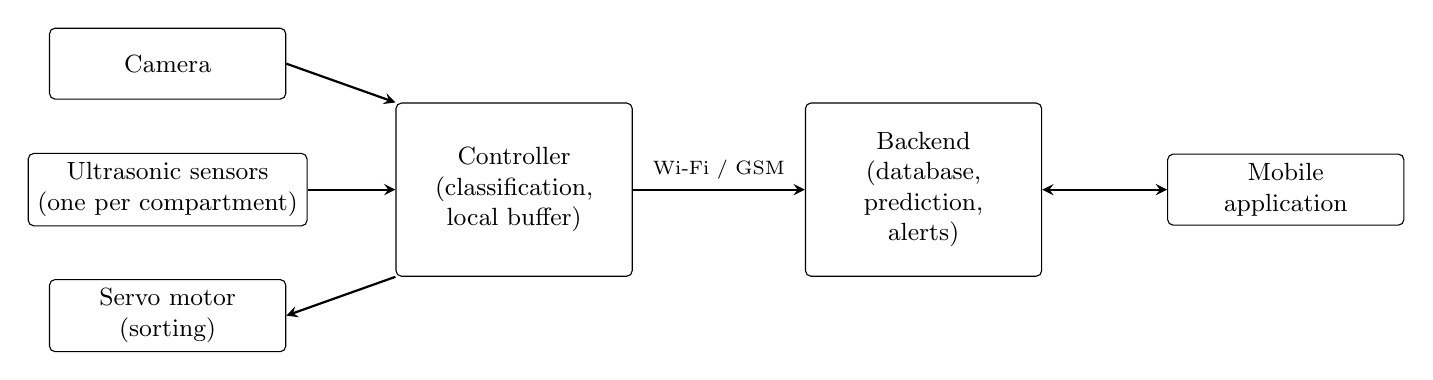
\begin{tikzpicture}[
  box/.style={draw, rounded corners=2pt, minimum width=3.0cm, minimum height=0.9cm, align=center, font=\small},
  arr/.style={->, >=stealth, thick}]
\node[box] (cam) at (0,3.2) {Camera};
\node[box] (us) at (0,1.6) {Ultrasonic sensors\\(one per compartment)};
\node[box] (servo) at (0,0) {Servo motor\\(sorting)};
\node[box, minimum height=2.2cm] (ctrl) at (4.4,1.6) {Controller\\(classification,\\local buffer)};
\node[box, minimum height=2.2cm] (back) at (9.6,1.6) {Backend\\(database,\\prediction,\\alerts)};
\node[box] (app) at (14.2,1.6) {Mobile\\application};
\draw[arr] (cam.east) -- (ctrl.north west);
\draw[arr] (us.east) -- (ctrl.west);
\draw[arr] (ctrl.south west) -- (servo.east);
\draw[arr] (ctrl.east) -- node[above, font=\scriptsize]{Wi-Fi / GSM} (back.west);
\draw[<->, >=stealth, thick] (back.east) -- (app.west);
\end{tikzpicture}}
\caption{Proposed system architecture}
\label{fig:arch}
\end{figure}

\subsection{Item handling flow}

When an item is placed in the input chamber, the controller checks whether the chamber holds an item. It captures an image and runs the classifier. If the class is confident and the matching compartment is not full, the servo directs the item there, the fill reading is updated and the reading is sent to the backend. Otherwise the item is held for manual checking and the application shows a notice. The backend adds the reading to the history, updates the prediction for that compartment and sends an alert if the threshold has been reached. A collector acknowledges the alert and later records the collection and the recipient.

\subsection{Hardware and software}

The hardware choices will be made during design. Candidates are a Raspberry Pi with its camera module as the main controller, an ESP32-CAM as a cheaper alternative, HC-SR04 ultrasonic sensors for fill level \cite{komane} and servo motors for sorting. We will compare the options on classification speed, power use and cost, using the comparison between the Jetson Nano and the K210 by Li and Grammenos \cite{li} as a guide. We will not assume that any sensor can tell organic waste from plastic on its own, so classification will be image based.

For the classifier we plan to use transfer learning from a small pre-trained model such as MobileNet \cite{li,white}, trained on TrashNet for the classes it covers and on our own images for food waste and for the empty and hand classes. The prediction component will start with the fill-rate baseline described in Chapter 1. If the data collected is enough, we will try an LSTM and a 1D CNN, which Ahmed et al. \cite{ahmed} found to give the lowest RMSE and the lowest MAPE respectively on bin data. The backend will use a database for readings and records and a message protocol suited to small devices. The mobile application will be built for Android and will show dashboards and push alerts.

\section{Implementation}

Implementation will follow the design in four steps. First we will collect and label the images and train the classifier. Second we will build the bin unit and connect the camera, sensors and servo. Third we will build the backend and the prediction component. Fourth we will build the mobile application and connect everything. Each step will be tested on its own before the parts are joined. The data we collect will be split into training, validation and test sets before any training starts, so that the test images are never used to tune the model.

\section{Testing and evaluation}

Testing will happen at three levels. Unit tests will check the individual functions, such as the fill-level calculation and the alert logic. Integration tests will check that the parts work together, for example that a reading from the controller reaches the application. System tests will check the prototype against the requirements in Tables~\ref{tab:fr} and~\ref{tab:nfr}.

The evaluation will use the parameters in Table~\ref{tab:params}. Classification will be evaluated on the held-out image set, and sorting success in physical trials with items from the participating sites. Fill-level error will be measured by comparing sensor readings with manual measurements. Prediction will be evaluated on later observations than those used for training and compared with the baseline. Alert delivery time will be measured from log timestamps, and task completion by asking a few staff and collectors to carry out set tasks with the application. The prototype will first be tested in a controlled setting and then, if access allows, in a supervised trial at one site. Results will be reported with their limitations, including the length of the data collection period.

\section{Ethical considerations}

We will ask for permission from each site before collecting any data and explain the purpose of the study to every participant. Participation will be voluntary and participants may withdraw at any time. Interview records will not carry names, and the names of sites will not be published without their agreement. The camera will be fixed to capture only the input chamber, and images in which a person appears will be deleted. Data will be stored securely and kept only as long as the project needs it.

\section{Risks and limitations}

Some sites may not agree to take part or may allow only a short observation period, which would limit the data for prediction. Food waste is harder to classify than the items in public datasets, and the classifier may do worse than the figures reported in the literature. Network and power at a site may be unreliable, which is why the bin stores readings locally. If any of these happens, we will report it as a limitation and reduce the scope of the field trial rather than claim results we have not measured.

\chapter{Work Plan}

Table~\ref{tab:plan} shows the planned activities over eight months. The months are counted from the start of the project, and the plan will be adjusted to the academic calendar once the dates are confirmed.

\begin{table}[htbp]
\centering
\small
\renewcommand{\arraystretch}{1.3}
\begin{tabular}{>{\raggedright\arraybackslash}p{6.4cm}*{8}{c}}
\hline
\textbf{Activity} & \textbf{1} & \textbf{2} & \textbf{3} & \textbf{4} & \textbf{5} & \textbf{6} & \textbf{7} & \textbf{8}\\
\hline
Study of the current situation & $\bullet$ & $\bullet$ & & & & & &\\
Requirements analysis & & $\bullet$ & & & & & &\\
Image collection and classifier training & & $\bullet$ & $\bullet$ & & & & &\\
System design & & & $\bullet$ & & & & &\\
Bin unit and backend implementation & & & $\bullet$ & $\bullet$ & $\bullet$ & & &\\
Mobile application & & & & $\bullet$ & $\bullet$ & & &\\
Integration and unit testing & & & & & $\bullet$ & $\bullet$ & &\\
Controlled and site testing & & & & & & $\bullet$ & $\bullet$ &\\
Evaluation and report writing & & & & & & & $\bullet$ & $\bullet$\\
\hline
\end{tabular}
\caption{Work plan by month}
\label{tab:plan}
\end{table}

\addcontentsline{toc}{chapter}{References}
\bibliographystyle{IEEEtran}
\bibliography{references}

\end{document}
